\subsection{Dati e risultati}

L'esperienza è stata divisa in varie parti. Abbiamo testato il funzionamento
di alcune porte logiche nella prima parte, verificato il loro comportamento
in commutazione nella seconda, e le abbiamo poi usate per montare un paio di
circuiti nella terza parte.

\paragraph{Porte logiche.}

Le porte che abbiamo utilizzato ci sono state fornite in forma di integrati contenenti
4 porte ciascuno. In elettronica digitale è comune lavorare con porte NAND poiché con
queste è possibile costruire quasi tutti gli altri tipi di porte facilmente; in questo
modo non è necessario avere molti tipi di integrati con le varie porte. Tutte le 
porte che abbiamo usato sono del tipo TTL, ovvero operano da 0 a + 5 V.

Abbiamo quindi verificato il funzionamento delle porte NAND sull'integrato 74LS00,
grazie ad una piccola schedina che mostra con dei LED il livello (alto o basso)
delle uscite.

Altre porte che abbiamo costruito e testato sono le porte NOT, AND e XOR,
la cui costruzione utilizzando porte NAND è riportata in figura \ref{fig:porte9}

\begin{figure}
    \centering
    \footnotesize
    \begin{subfigure}{0.44\columnwidth}
        \centering
        \begin{circuitikz}
            \draw
                (1.75, 0) node[american nand port] (nand1) {}
                (nand1.in 1) to (nand1.in 2) 
                (0, 0) node [anchor=east] {IN} -| (nand1.in 1)
                (nand1.out) node [anchor=west] {OUT}
            ;
        \end{circuitikz}
        \caption{NOT}
        \label{fig:not9}
    \end{subfigure}
    \begin{subfigure}{0.54\columnwidth}
        \centering
        \begin{circuitikz}
            \draw
                (1.75, 0) node[american nand port] (nand1) {}
                (3.5, 0) node[american nand port] (nand2) {}
                (nand1.out) -| (nand2.in 1)
                (nand1.out) -| (nand2.in 2)
                (nand1.in 1) node [anchor=east] {A}
                (nand1.in 2) node [anchor=east] {B}
                (nand2.out) node [anchor=west] {OUT}
            ;
        \end{circuitikz}
        \caption{AND}
        \label{fig:and9}
    \end{subfigure}
    \begin{subfigure}{\columnwidth}
        \centering
        \begin{circuitikz}
            \draw
                (1, 0) node[american nand port] (nand1) {}
                (3, 1) node[american nand port] (nand2) {}
                (3, -1) node[american nand port] (nand3) {}
                (5, 0) node[american nand port] (nand4) {}
                (nand1.out) -| (nand2.in 2)
                (nand1.out) -| (nand3.in 1)
                (nand2.out) -| (nand4.in 1)
                (nand3.out) -| (nand4.in 2)
                (nand2.in 1) to ++ (-2.5, 0) node [anchor=east] {A}
                (nand3.in 2) to ++ (-2.5, 0) node [anchor=east] {B}
                (nand1.in 1) to ++ (0, 1)
                (nand1.in 2) to ++ (0, -1)
                (nand4.out) node [anchor=west] {OUT}
            ;
        \end{circuitikz}
        \caption{XOR}
        \label{fig:xor9}
    \end{subfigure}
    \caption{Tutte le altre porte logiche possono essere costruite utilizzando porte NAND.
	Per una NOT (\ref{fig:not9}) è sufficiente collegare tra di loro gli ingressi,
	la AND si ottiene mettendo una NAND in serie ad un NOT, per rovesciare lo stato logico,
	mentre una XOR è un poco più complicata, ma sempre realizzabile con poche porte NAND.
	Anche la OR non è difficile da realizzare, con due not agli ingressi di una NAND.}
    \label{fig:porte9}
\end{figure}

\paragraph{Isteresi della porta NOT.}

Ogni componente digitale ha delle bande di tensione che vengono trattate come 0 e 1 logici. Per esempio
una porta logica può considerare 0 le tensioni più basse di una certa soglia (nella TTL, 0.8 V), 
e 1 le tensioni superiori ad un altra soglia (nella TTL, 2 V). La banda a metá tra le due soglie
dà un risultato indefinito. Tuttavia le soglie non sono fisse, ma dipendono se si sta salendo o
scendendo di tensione, ovvero è presente un ciclo di isteresi. Inoltre questi dispositivi
devono rispondere ad uno standard che prevede che la loro uscita per i livelli logici 0 e 1 sia
contenuta in certe bande di tensione. Noi non abbiamo verificato quest'ultimo aspetto.

\begin{figure}[b!]
    \centering
    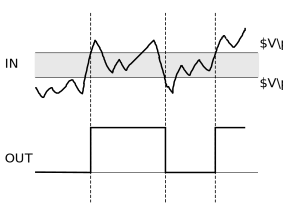
\includegraphics[width=\columnwidth]{figure/ist.pdf}
    \caption{Il grafico mostra l'isteresi della porta NOT. L'ampiezza dell'isteresi è di circa 0.1 V e avviene attorno a 1.1 V.
        Questo significa che partendo da 0 V e salendo in tensione, si ha la commutazione a circa 1.15 V, mentre
        scendendo da 5 V la commutazione avviene a circa 1.05 V. La tensione alta non è sempre 5 V, anzi in base alla tensione di ingresso
        l'output varia visibilmente.}
    \label{fig:ist9}
\end{figure}

Per verificare l'esistenza dell'isteresi
abbiamo collegato l'ingresso della porta NOT al generatore di tensione, variando poco a poco la tensione
di ingresso e misurando l'uscita. In questo modo abbiamo ottenuto il grafico in figura \ref{fig:ist9}.

Il grafico mostra che quando la tensione di ingresso sale, l'output è differente rispetto alla stessa situazione
registrata durante la discesa della tensione di input. Vale a dire che la commutazione alto-basso non è simmetrica
dipende dallo stato precedente della porta logica. Inoltre possiamo notare che la tensione che rappresenta lo stato
1 è tutt'altro che costante, dipende dall'input in maniera approssimativamente lineare tra le tensioni da 4.5 a 3.5 V.

\paragraph{Votazioni.}

\begin{figure}
    \centering
    \begin{circuitikz}[scale=0.65, transform shape]
        % Parte sopra
        \draw
        (2, 3) node[american nand port] (nand1A) {}
        (2, 1) node[american nand port] (nand1B) {}
        (4, 2) node[american nand port] (nand1C) {}
        (5, 2) node[american not port] (not1) {}
        (nand1A.out) -| (nand1C.in 1)
        (nand1B.out) -| (nand1C.in 2)
        (nand1C.out) -- (not1.in)
        (nand1A.in 2) -- ++(-2,0) node[left]{A}
        (nand1B.in 2) -- ++(-2,0) node[left]{B}
        (nand1A.in 1) ++(-2,0) node[left]{P} -| (nand1B.in 1)
        ;
        
        % Prima parte sotto
        \draw
        (2, -1) node[american nand port] (nand2) {}
        (2, -3) node[american not port] (not2) {}
        (nand1A.in 1) ++(-0.3,0) |- (nand2.in 1)
        (nand1B.in 2) ++(-0.6,0) |- (nand2.in 2)
        (nand1A.in 1) ++(-0.9,0) |- (not2.in)
        ;
         
        % Seconda parte sotto
        \draw
        (4.5, -2) node[american nand port] (nand3A) {}
        (6.5, -3) node[american nand port] (nand3B) {}
        (nand2.out) -| (nand3A.in 1)
        (not2.out) -| (nand3A.in 2)
        (nand3A.out) -| (nand3B.in 1)
        (nand3B.in 2) -- ++(-1,0) node[left]{C}
        ;
        
        % Unione
        \coordinate (U) at ($ (nand3B.out) !0.5! (not1.out) $); % !0.5! moltiplica per 0.5
        \draw
        (U) ++ (3,0) node [american nand port] (nand4) {}
        (not1.out) -| (nand4.in 1)
        (nand3B.out) -| (nand4.in 2)
        (nand4.out) -- ++(0.5,0) node[right]{OUT}
        ;
    \end{circuitikz}
    \caption{}
    \label{fig:circ_vota9}
\end{figure}

Nell'ultima parte dell'esperienza abbiamo costruito due circuiti come applicazione delle
porte logiche. Il primo circuito calcola il risultato di una votazione
in cui possono votare 3 persone (A, B e C) più il presidente (P), con la particolarità
poco democratica che il voto del presidente vale doppio. Il circuito prende quindi 4 input (i voti),
che sono a 0 se la voto è contrario e 1 se è favorevole all'emendamento in votazione.

\begin{table}
    \centering
    \footnotesize
    \begin{tabular}{c c c c | c || c c c c | c}
        \toprule
        A & B & C & P & OUT &  A & B & C & P & OUT \\
	\midrule
        0 & 0 & 0 & 0 & 0 & 0 & 0 & 0 & 1 & 0 \\
        0 & 0 & 1 & 0 & 0 & 0 & 0 & 1 & 1 & 1 \\
        0 & 1 & 0 & 0 & 0 & 0 & 1 & 0 & 1 & 1 \\
        0 & 1 & 1 & 0 & 0 & 0 & 1 & 1 & 1 & 1 \\
        1 & 0 & 0 & 0 & 0 & 1 & 0 & 0 & 1 & 1 \\
        1 & 0 & 1 & 0 & 0 & 1 & 0 & 1 & 1 & 1 \\
        1 & 1 & 0 & 0 & 0 & 1 & 1 & 0 & 1 & 1 \\
        1 & 1 & 1 & 0 & 1 & 1 & 1 & 1 & 1 & 1 \\
        \bottomrule
    \end{tabular}
    \caption{Tabella di verità del circuito per la votazione che abbiamo realizzato.
        A, B e C sono i votanti, mentre P è il presidente. La tabella è spezzata per questioni di spazio.}
    \label{tab:vota9}
\end{table}

\begin{table}
    \centering
    \begin{tabular}{c | c c c c}
		\toprule
        CP-AB & 00 & 01 & 11 & 10 \\
        \midrule
        00 & 0 & 0 & 0 & 0 \\
        01 & 0 & \marktopleft{c2}1 & \marktopleft{c3}1 & \marktopleft{c4}1 \\
        11 & \marktopleft{c1}1 & 1\markbottomright{c2} & \marktopleft{c5}1\markbottomright{c3} & 1\markbottomright{c1}\markbottomright{c4} \\
        10 & 0 & 0 & 1\markbottomright{c5} & 0 \\
		\bottomrule
    \end{tabular}
    \caption{Mappa di Karnaugh della tabella \ref{tab:vota9}, con cerchiati i gruppi che 
		permettono di scrivere l'equazione \ref{eq:logic9}.}
    \label{tab:karnaugh_vota9}
\end{table}

La tabella di verità che vogliamo ottenere è la \ref{tab:vota9} e come
si nota tende verso la dittatura del presidente. Dalla tabella si può costruire la
mappa di Karnaugh corrispondente (tabella \ref{tab:karnaugh_vota9}). Raggruppando sulla mappa i gruppi di celle vicine,
si ottiene l'espressione logica corrispondente alla tabella:

\begin{equation}
	Y = P(A + B + C) + ABC
	\label{eq:logic9}
\end{equation}

Che può essere scritta mediante NOT e AND (e quindi NAND) applicando ripetutamente il
teorema di De Morgan

\begin{equation}
	Y = \overline{\overline{P(\overline{\overline{A} \cdot \overline{B} \cdot \overline{C}})} \cdot \overline{ABC}}
\end{equation}

In questo modo è possibile costruire un circuito che produca il risultato desiderato mediante
sole porte NAND. Il circuito che rispetta questa logica è mostrato in figura \ref{fig:circ_vota9}
ed è quello che siamo andati a realizzare. Il circuito è stato controllato utilizzando la
scheda che permette di visualizzare con dei LED lo stato logico delle uscite, e possiamo
dire che è stato un successo perché lo abbiamo montato correttamente al primo colpo, nonostante
il circuito sia abbastanza complesso.

\paragraph{Sistema di allarme.}

Un secondo circuito è un altro esercizio che riguarda un allarme antifurto per una casa.
L'idea è quella di avere vari sensori che indicano se le porte o finestre sono aperte o chiuse e
un altro sensore ad infrarossi che indica la presenza di movimento in una stanza a scelta.
Il sensori restituiscono uno 0 logico se le porte e finestre sono chiuse o se il sensore a infrarossi
non rileva movimento e 1 in caso contrario. Ognuno dei tre sensori può far scattare l'allarme,
ma il sensore a infrarossi è dotato anche di un interruttore o di una chiave che permette di disattivarlo.

Partendo da queste specifiche, costruendo la tabella di verità ed utilizzando il metodo della mappa
di Karnaugh come nel paragrafo precedente, è possibile ricavare la seguente espressione logica che
ottiene quello che vogliamo

\begin{equation}
	Y = I\overline{C} + F + P = \overline{\overline{I}C \cdot (\overline{F}\cdot\overline{P})}
\end{equation}
%
dove ovviamente P indica la porta, F la finestra, I il sensore ad infrarossi e C la chiave per disattivare
l'allarme con gli infrarossi. Questa espressione è anche intuitiva: o la finestra aperta, o la porta aperta,
oppure il sensore ad infrarossi, se la chiave non è inserita. Il circuito corrispondente è mostrato in \ref{fig:allarme9}.

\begin{figure}
    \centering
    \footnotesize

        \begin{circuitikz}
            \draw
                (1.8, 0) node[nand port] (nand1) {}
				(1.8, 2) node[nand port] (nand2) {}
				(1.8, 4) node[nand port] (nand3) {}
				(0, 0) node[anchor=east] {F} -| (nand1.in 1)
				(0, 0) -| (nand1.in 2)
				(0, 2) node[anchor=east] {P} -| (nand2.in 1)
				(0, 2) -| (nand2.in 2)
				(0, 4) node[anchor=east] {C} -| (nand3.in 1)
				(0, 4) -| (nand3.in 2)
				(3.5, 5) node[nand port] (nand4) {}
				(3.5, 1) node[nand port] (nand5) {}
				(5, 1) node[nand port] (nand6) {}
				(nand1.out) -| (nand5.in 2)
				(nand2.out) -| (nand5.in 1)
				(0, 6) node[anchor=east] {I} -| (nand4.in 1)
				(nand3.out) -| (nand4.in 2)
				(nand5.out) -| (nand6.in 1)
				(nand5.out) -| (nand6.in 2)
				(7, 3) node[nand port] (nand7) {}
				(nand6.out) -| (nand7.in 2)
				(nand4.out) -| (nand7.in 1)
				(nand7.out) node[anchor=west] {OUT}
            ;
        \end{circuitikz}
    \caption{}
    \label{fig:allarme9}
\end{figure}

La verifica del circuito è banale ed è andata a buon fine.
